\documentclass{uofa-eng-assignment}

\usepackage{lipsum}
\usepackage{graphicx}

\newcommand*{\name}{Mohammad Mohammad Beigi}
\newcommand*{\id}{99102189}
\newcommand*{\subject}{Convex Optimization}
\newcommand*{\course}{Convex Optimization}
\newcommand*{\assignment}{Assignment 1}
\lstset{ 
	language=Matlab,                		% choose the language of the code
	%	basicstyle=10pt,       				% the size of the fonts that are used for the code
	numbers=left,                  			% where to put the line-numbers
	numberstyle=\footnotesize,      		% the size of the fonts that are used for the line-numbers
	stepnumber=1,                   			% the step between two line-numbers. If it's 1 each line will be numbered
	numbersep=5pt,                  		% how far the line-numbers are from the code
	%	backgroundcolor=\color{white},  	% choose the background color. You must add \usepackage{color}
	showspaces=false,               		% show spaces adding particular underscores
	showstringspaces=false,         		% underline spaces within strings
	showtabs=false,                 			% show tabs within strings adding particular underscores
	%	frame=single,	                			% adds a frame around the code
	%	tabsize=2,                				% sets default tabsize to 2 spaces
	%	captionpos=b,                   			% sets the caption-position to bottom
	breaklines=true,                			% sets automatic line breaking
	breakatwhitespace=false,        		% sets if automatic breaks should only happen at whitespace
	escapeinside={\%*}{*)}          		% if you want to add a comment within your code
}

\begin{document}

\maketitle

\section*{Question 1}

$\sqrt{x}$ is concave for $x > 0$.\\
$\frac{1}{u}$ is convex for $u > 0$\\
So by DCP rules, $\frac{1}{\sqrt{x}}$ is concave.

The Function $g(x, y) = \frac{x^2}{y}$ is jointly convex for $x,y > 0$.(increasing for $x>0$ and decreasing for $ y > 0$.

So by DCP and general vector composition rules:
\[
g(\frac{1}{\sqrt{x}}, y) = \frac{\frac{1}{\sqrt{x}^2}}{y} = \frac{1}{xy}
\]
is convex.

\section*{Question 2}

\subsection*{part a}

Minimizing the sum of the disk areas:
\[
\text{First objective Function } \sum_{i=1}^{n} \pi r_i^2
\]
Minimizing
sum of the disk
perimeters:
\[
\text{Second objective Function } \sum_{i=1}^{n} 2\pi r_i
\]
These are convex functions because we have: $r_i > 0$ \\
1st constraint: First k disks are fixed. $\rightarrow$ set of linear constraints $\Rightarrow$ convex\\
2nd constraint: $\lVert c_i -c_j \rVert_2 \le r_i+r_j$ for each (i, j) $\in$ I $\Rightarrow$ $\lVert c_i -c_j \rVert_2 - (r_i+r_j) \le 0$\\
$\lVert c_i -c_j \rVert_2$ is constant and $r_i+r_j$ is linear. $\Rightarrow$ convex\\
So:


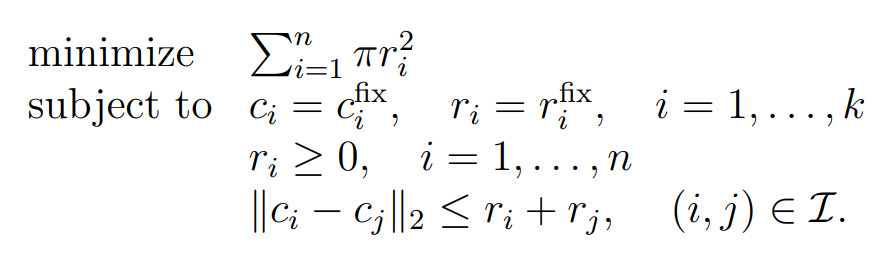
\includegraphics[width=0.5\linewidth]{screenshot003}
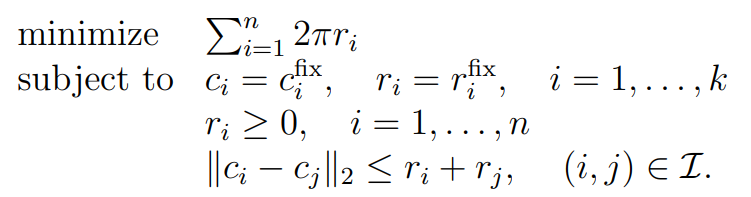
\includegraphics[width=0.5\linewidth]{screenshot004}

\subsection*{part b}

Results are as below:

\begin{center}
	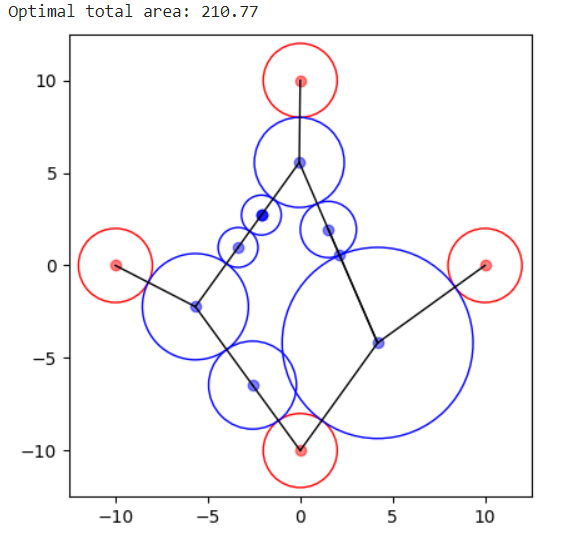
\includegraphics[width=0.6\linewidth]{screenshot005}
\end{center}


\begin{center}
	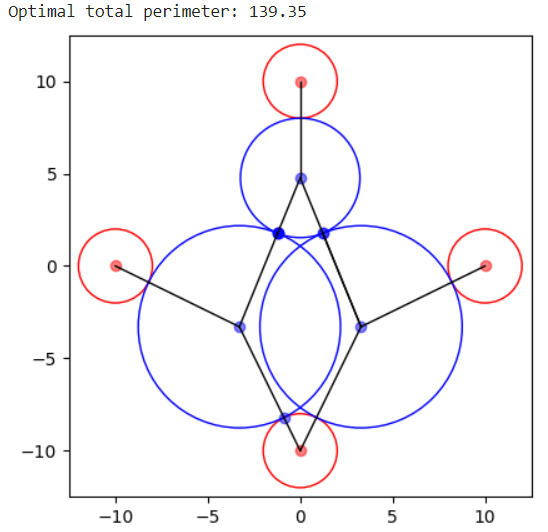
\includegraphics[width=0.58\linewidth]{screenshot006}
\end{center}

Minimizing the Perimeter:

The perimeter here refers to the total boundary length of all the disks.
The text notes that when minimizing the perimeter, which is essentially the sum of the radii of the disks (also referred to as the '1 norm' since it involves the sum of absolute values), the resulting solution tends to have a few disks with large radii and several disks with zero radii.
This behavior is characterized as typical of 'L1 minimization,' where the optimization process tends to prioritize a sparse set of larger values (disks with large radii) while allowing others to be eliminated (disks with zero radii).


Minimizing the Area:

The area in this context is the sum of the squares of the radii of the disks (referred to as the 'L2 norm squared').
When minimizing the area, the solution tends to have fewer disks with large radii, and importantly, none of the disks have zero radii.
This behavior is associated with 'L2 minimization,' where the optimization process distributes the values more evenly, avoiding complete elimination (zero radii) and favoring a balance among the radii.

In summary, the choice of the objective function (minimizing perimeter or area) influences the distribution of radii among the disks. Minimizing the perimeter tends to result in a solution with a few large disks and several with zero radii, while minimizing the area leads to a solution with fewer large disks and none with zero radii. The choice between L1 and L2 norms reflects different optimization preferences and trade-offs in the system.

\section*{Question 3}

\subsection*{part a}

\[
\hat{y} = Ax
\]
$x = (a, b)\in R^{2B}$ is a vector of
cosine and sinusoid coefficients and $A = [C, S] \in R^{n\times2B}$ with $C,S \in R^{n\times B}$ and:
\[
C_{tj} = \cos(2\pi(f_{min}+j-1)\frac{t}{n})
\]
\[
S_{tj} = \sin(2\pi(f_{min}+j-1)\frac{t}{n})
\]

Let $s_ta_t^Tx\ge0$  where $a_i^T$ is i-th row of A, to ensure that the signs of $\hat{y}$ are consistent with s.

Linear equality constraint:
$\lVert \hat{y} \rVert_1 = s^TAx = n$

(The signs are given so this constraint is convex in general)

So:

\begin{center}
	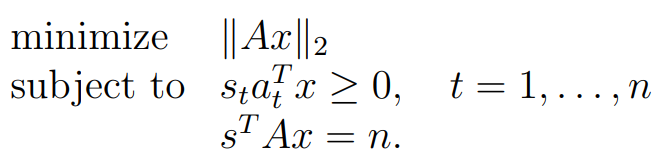
\includegraphics[width=0.4\linewidth]{screenshot008}
\end{center}

Suppose that $x^\star$ is the solution of the problem. So the min  value is $y^\star = Ax^\star$.\\
A prevalent error involved approaching the aforementioned problem without incorporating the normalization constraint. The flawed rationale behind this approach was the idea of solving the homogeneous problem first, followed by scaling the result to ensure its $l_1$ norm is one. However, this approach proves ineffective, as the sole solution to the homogeneous problem is x = 0 (given that x = 0 is feasible). Surprisingly, despite this, the method yielded numerical outcomes significantly superior to x = 0. This can be attributed to the fact that the solvers produced a minute x, for which Ax exhibited the correct sign. It's important to note that this does not imply the absence of a substantial error.






\subsection*{part b}
\begin{center}
	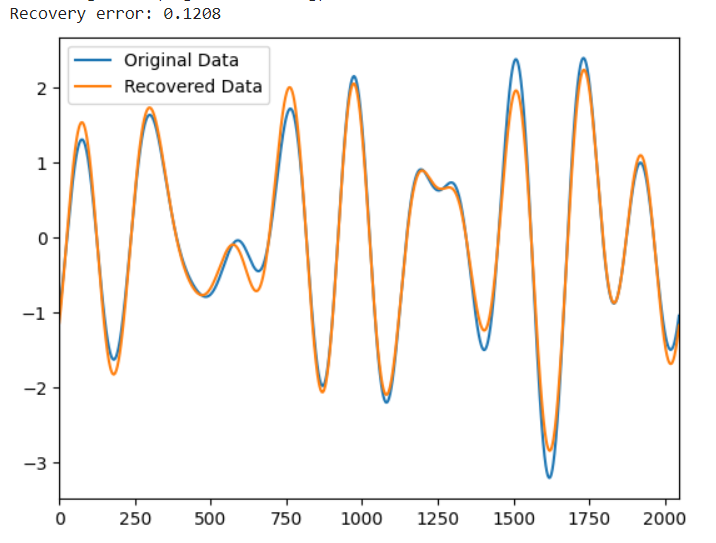
\includegraphics[width=0.6\linewidth]{screenshot007}
\end{center}

The recovery error stands at 0.1208, and it's remarkably impressive, considering the scant information we had at our disposal.


\section*{Question 4}

\subsection*{part a}
\[
Pr(N_t \text{ events occur}) = e^{-\lambda_t} \frac{\lambda_t^{N_t}}{(N_t)!} \Rightarrow \log (Pr(N_t \text{ events occur})) = -\lambda_t + N_t \log (\lambda_t) - \log(N_t!)
\]

So log-likelihood of collection of $N_t$s is :
\[
LR = \prod_{t=1}^{24} Pr(N_t \text{ events occur}) =  \sum_{t=1}^{24}  -\lambda_t + N_t \log (\lambda_t) - \log(N_t!) 
\]
So we should minimize negative log-likelihood:
\[
\frac{\partial (-LR)}{\partial \lambda_t} = 1 - \frac{N_t}{\lambda_t} = 0 \Rightarrow \lambda_t = N_t
\]
This means
if you observe $N_t$ events, you will
guess that this is the mean of the number of events that occur.


\subsection*{part b}

We should solve the convex optimization problem

\[
\text{minimize} \sum_{t=1}^{24}  \lambda_t - N_t \log (\lambda_t) + \log(N_t!) + \rho (\sum_{t=1}^{23} (\lambda_t-\lambda_{t+1})^2 +(\lambda_{24} - \lambda_1)^2);\textbf{subject to } \lambda,\rho \ge 0\textbf{ , } \lambda\in R^{24}
\]
Let's call the function above f.

\subsection*{part c}
As $\rho\to\infty$, since we should let $\frac{\partial f}{\partial \rho} = 0$ we get 
\[
(\sum_{t=1}^{23}\lambda_t-\lambda_{t+1})^2 +(\lambda_{24} - \lambda_1)^2 = 0 \Rightarrow \text{all } \lambda_ts \text{ are equal}
\]

So we should minimize the following function:
\[
\sum_{t=1}^{24}  \hat{\lambda} - N_t \log (\hat{\lambda}) + \log(N_t!) 
\]
which is equal to minimizing the following function:
\[
g(\lambda) = \sum_{t=1}^{24}  \hat{\lambda} - N_t \log (\hat{\lambda}) = 24\hat{\lambda} - \log (\hat{\lambda}) \sum_{t=1}^{24}  N_t 
\]
\[
\frac{\partial g(\lambda)}{\partial \lambda} = 24 - \frac{\sum_{t=1}^{24} N_t}{\hat{\lambda}} = 0 \Rightarrow \hat{\lambda} = \frac{\sum_{t=1}^{24} N_t}{24}
\]

So the solution is the constant Poisson model $\hat{\lambda} = \frac{\sum_{t=1}^{24} N_t}{24}$. 

\subsection*{part d}

The estimated rates are as below:

\begin{center}
	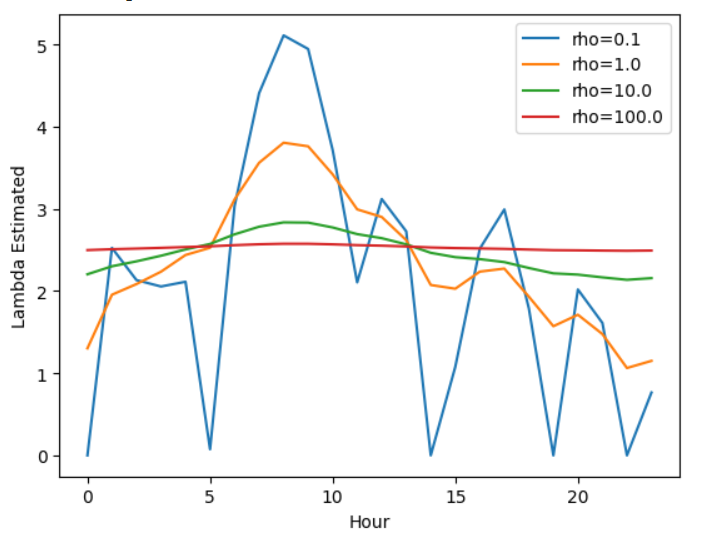
\includegraphics[width=0.65\linewidth]{screenshot001}
\end{center}

(You can observe that the larger $\rho$ is, the smoother
$\lambda$ is.)

\subsection*{part e}

\begin{center}
	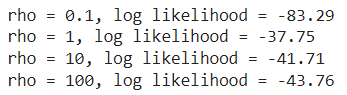
\includegraphics[width=0.5\linewidth]{screenshot002}
\end{center}
By the log-likelihood for rhos shown above,
we would choose $\rho = 1$, since it gets the highest log-likelihood on the test set.


\end{document}
